% ============================================================
% Kapitola 5 — Diskuse a~rozšíření modelu
% ============================================================
\chapter{Diskuse a~rozšíření modelu}
\label{chap:diskuse}

V~předchozí kapitole jsme prezentovali baseline výsledky stochastické
simulace pro~čtyři kvality půdy a~dvě plodiny. Cílem této kapitoly
je~rozšířit baseline o~klíčové \emph{rozšiřující scénáře}, které mění
jednu z~axiomatických podmínek modelu, a~diskutovat, \emph{jak} a~\emph{kolik}
rizikový profil reaguje. Postupně analyzujeme:
\begin{enumerate}
    \item vliv \textbf{dotační podpory} CAPEX (\S~\ref{sec:dotace}),
    \item dopad \textbf{katastrofického klimatického scénáře} ---
          desetiletí systémově snížených výnosů (\S~\ref{sec:katastrofa}),
    \item potenciál \textbf{diverzifikace portfolia} při kombinaci obou
          plodin (\S~\ref{sec:diverzifikace}),
    \item \textbf{limitace modelu} a~doporučení pro~budoucí výzkum
          (\S~\ref{sec:limitace}).
\end{enumerate}

Každá ze~sekcí staví na~baseline z~kapitoly~\ref{chap:vysledky}, takže
\emph{všechny rozdíly} se~hodnotí vůči baseline tabulkám
\ref{tab:nevhodna-metriky}--\ref{tab:optimalni-metriky}.

% ============================================================
\section{Vliv dotací na~CAPEX}
\label{sec:dotace}

V~baseline analýze byl dotační podíl nastaven na~$0~\%$, aby~odrážel
\emph{nejhorší možný scénář} pro~pěstitele bez~přístupu k~veřejné
podpoře. V~realitě se~však pěstování energetických plodin v~ČR opírá
o~několik nástrojů: SZP (Strategický plán SZP 2023--2027) přiznává
\textbf{přímé platby} a~\textbf{ekoschémata}, Modernizační fond podporuje
investice do~biomasových zdrojů a~od~roku 2025 platí Vyhláška
315/2025~Sb., která pevně stanovuje \emph{garantovanou
kupní cenu} pro~biomasové zdroje a~tím nepřímo dotuje provoz
plantáže. Pro~účely této práce kvantifikujeme vliv \emph{kapitálové dotace}
ve~formě podílu \(s\) \% celkového CAPEXu, kalibrovaného v~kapitole~\ref{chap:metodologie}.
Cílem této sekce \emph{není} fiskální analýza dotačních titulů
v~ČR, nýbrž posouzení, jak~dotace mění \emph{rizikový profil}
investice — tedy variabilitu, dolní chvost a~pravděpodobnost
ziskovosti, nikoli pouze střední hodnotu.

\paragraph{Konfigurace experimentu.}
Spustili jsme totožnou simulaci jako v~kapitole~\ref{chap:vysledky}
(${N = 10\,000}$, $10$~ha, pacht $200$~EUR/ha/rok, $r = 0~\%$) pro~čtyři
úrovně dotace na~CAPEX: \(s \in \{0, 25, 50, 75\}~\%\). Dotace zasahuje
\emph{pouze} kapitálovou výdajovou položku v~roce výsadby
(\(t = 1\)) a~v~případě obnovy plantáže po~selhání
($t = 1$, $0{,}6 \cdot \mathrm{CAPEX}$). Provozní náklady,
likvidace ani daň z~pozemku dotovány nejsou.

\subsection{Výsledky -- posun střední hodnoty}
\label{subsec:dotace-mean}

Tabulka~\ref{tab:dotace-shrnuti} prezentuje EAA a~klíčové rizikové
ukazatele pro~všechny kombinace půda \(\times\) plodina v~baseline
\((s = 0)\) a~variantě \(s = 50~\%\). Plný citlivostní průběh všech
čtyř hladin dotace zachycuje obrázek~\ref{fig:dotace-citlivost}.

\begin{table}[H]
\centering
\caption{Vliv dotace 50~\% CAPEX na~rizikový profil
(\(N = 10\,000\), 10~ha, pacht 200~EUR/ha/rok, \(r = 0~\%\)).}
\label{tab:dotace-shrnuti}
\renewcommand{\arraystretch}{1.15}
\small
\begin{tabular}{ll|rrr|rrr}
\toprule
\multicolumn{2}{c|}{} & \multicolumn{3}{c|}{\textbf{Bez dotace}} & \multicolumn{3}{c}{\textbf{Dotace 50~\%}} \\
\textbf{Půda} & \textbf{Plodina} & $\mu_{\mathrm{EAA}}$ & $P(\!+\!)$ & CVaR$_{5\%}$ & $\mu_{\mathrm{EAA}}$ & $P(\!+\!)$ & CVaR$_{5\%}$ \\
\midrule
Nevhodná   & Miscanthus & $-3\,715$ & $0~\%$    & $-4\,843$ & $-3\,115$ & $0~\%$    & $-4\,183$ \\
           & SRC vrba   & $-2\,565$ & $0~\%$    & $-3\,352$ & $-2\,340$ & $0~\%$    & $-3\,117$ \\
\midrule
Neúrodná   & Miscanthus & $-1\,945$ & $0{,}1~\%$  & $-3\,080$ & $-1\,346$ & $1{,}3~\%$  & $-2\,424$ \\
           & SRC vrba   & $-1\,049$ & $1{,}4~\%$  & $-1\,905$ & $-824$    & $3{,}5~\%$  & $-1\,669$ \\
\midrule
Průměrná   & Miscanthus & $+589$    & $67{,}2~\%$ & $-1\,676$ & $+1\,189$ & $83{,}0~\%$ & $-1\,049$ \\
           & SRC vrba   & $+1\,250$ & $92{,}1~\%$ & $-576$    & $+1\,476$ & $95{,}0~\%$ & $-346$ \\
\midrule
Optimální  & Miscanthus & $+2\,871$ & $97{,}1~\%$ & $-515$    & $+3\,470$ & $97{,}4~\%$ & $+94$ \\
           & SRC vrba   & $+3\,159$ & $97{,}5~\%$ & $+298$    & $+3\,384$ & $97{,}5~\%$ & $+526$ \\
\bottomrule
\end{tabular}
\end{table}

\begin{figure}[H]
\centering
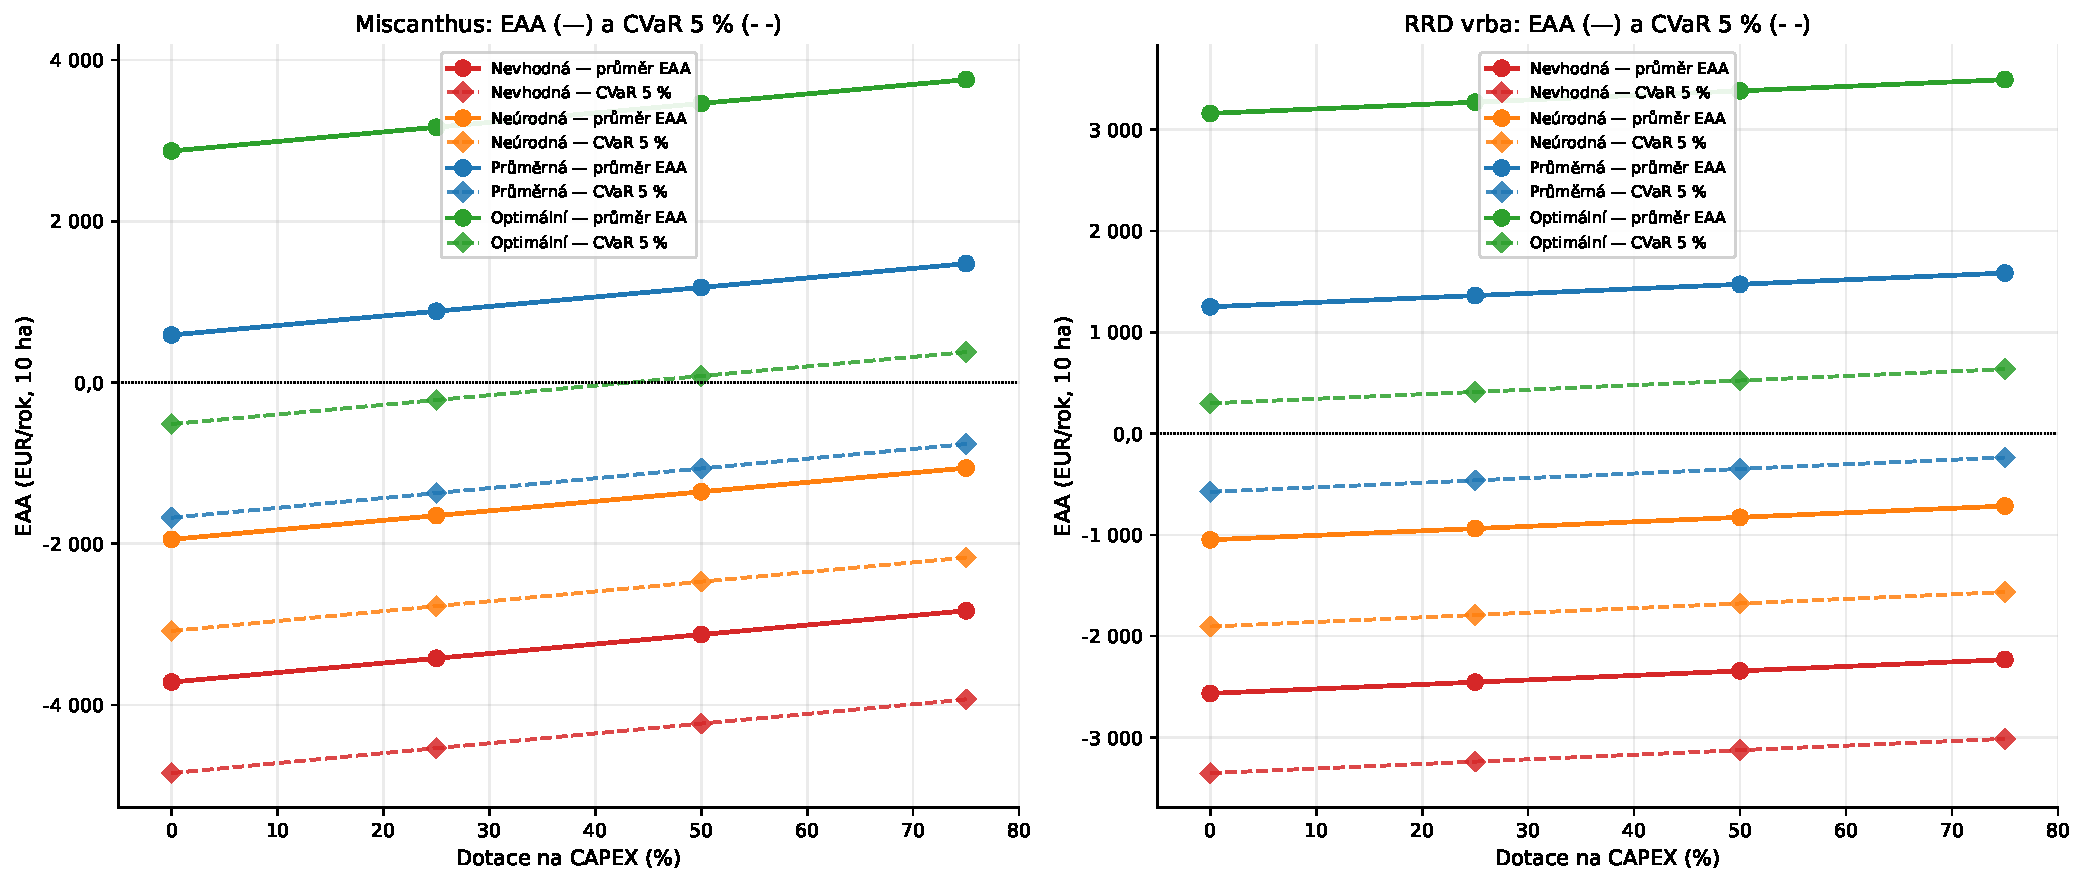
\includegraphics[width=\textwidth]{img/kap05/05_dotace_citlivost.pdf}
\caption{Citlivost průměrné EAA (plné čáry) a~CVaR$_{5\%}$ (čárkované)
na~míru dotace CAPEX 0--75~\%. Dotace zvyšuje obě veličiny prakticky
\emph{lineárně} a~\emph{paralelně} -- mezera mezi $\mu$ a~CVaR
(rezerva proti chvostové ztrátě) zůstává konstantní.}
\label{fig:dotace-citlivost}
\end{figure}

\paragraph{Klíčové pozorování -- konstantní translační efekt.}
Zvýšení dotace o~$25$ procentních bodů zvyšuje průměrnou EAA \emph{nezávisle
na~kvalitě půdy} přibližně o~$+300$~EUR/rok pro~Miscanthus
a~$+113$~EUR/rok pro~SRC vrbu. Důvod je~prostý: kapitálová dotace
je~deterministický \emph{translační operátor} aplikovaný na~jedinou
položku CAPEX v~roce 1 -- v~modelu nemá žádný stochastický rozměr.
Posun anuity činí
\[
\Delta \mathrm{EAA} \;=\; \frac{s \cdot \mathrm{CAPEX}}{n_{\mathrm{life}}},
\qquad s \in [0,1],
\]
což pro~Miscanthus s~CAPEX $\approx 3\,000$~EUR/ha a~$n = 25$ dává
$\Delta \mathrm{EAA} \approx 60 \cdot s$ EUR/ha/rok, tj.~$+150$~EUR/rok
pro~$s = 0{,}25$ při 10~ha — a~empiricky pozorovaný posun
$\sim +300$~EUR/rok zahrnuje navíc i~úsporu z~očekávaných obnov
plantáže (riziko $5~\%$, $60~\%$ obnoveno). Pro~SRC s~nižším CAPEX
($\sim 1\,400$~EUR/ha) a~$n = 30$ je~efekt slabší.

\subsection{Výsledky -- variabilita a~chvost}
\label{subsec:dotace-rizika}

Pro~komplexní obraz však \emph{střední hodnota nestačí}. Vyhodnocujeme
proto vliv dotace samostatně na~tři rizikové ukazatele:
\begin{itemize}
\item \textbf{$\sigma_{\mathrm{CF}}^{\mathrm{rok}}$} (variabilita
      ročního cash flow) zůstává \emph{nezměněna} ve~všech kombinacích
      (rozdíl pod~1~\%), protože dotace ovlivňuje pouze \emph{deterministickou}
      složku CF v~roce 1.
\item \textbf{CVaR$_{5\%}$ EAA} se~posouvá o~stejné absolutní množství
      jako střední hodnota -- gap $\mu - \mathrm{CVaR}$, který kvantifikuje
      \emph{hloubku chvostového scénáře relativně k~průměru},
      zůstává konstantní (cca~$1\,100$ EUR/rok pro~Miscanthus,
      $1\,800$ EUR/rok pro~SRC).
\item \textbf{Pravděpodobnost ziskovosti $P(\mathrm{EAA} > 0)$}
      reaguje \emph{nelineárně}: největší přírůstek nastává tam, kde
      baseline distribuce má~modu blízko nuly. Pro~Miscanthus
      na~průměrné půdě $P(+)$ stoupá z~$67{,}2~\%$ (bez dotace) na~$83{,}0~\%$ (50~\%);
      naopak na~optimální půdě $P(+) \approx 97~\%$ je~dotací prakticky
      nasycena.
\end{itemize}

\noindent\textbf{Praktická interpretace.} Dotace 50~\% CAPEX
\emph{neeliminuje} riziko, ale~\emph{posune celou distribuci EAA o~konstantní
hodnotu doprava}. Vypovídá tedy o~\emph{dotování průměrné výnosnosti},
nikoli o~snížení rizikového profilu. Tento efekt je~v~kontrastu s~ostatními
nástroji veřejné podpory, jako jsou \emph{garantované výkupní ceny}
(Vyhláška 315/2025~Sb.) nebo \emph{pojištění proti ztrátě úrody}, které
by~přímo snižovaly $\sigma_{\mathrm{CF}}$ a~ohraničovaly chvost rozdělení.
Modelování těchto nástrojů je~nad~rámec této práce, ale~představuje
přirozené pokračování (viz~\S~\ref{sec:limitace}).

Obrázek~\ref{fig:dotace-eaa-prumerna} demonstruje translační efekt
na~průměrné půdě, kde dotace nejvýrazněji ovlivňuje pravděpodobnost
ziskovosti.

\begin{figure}[H]
\centering
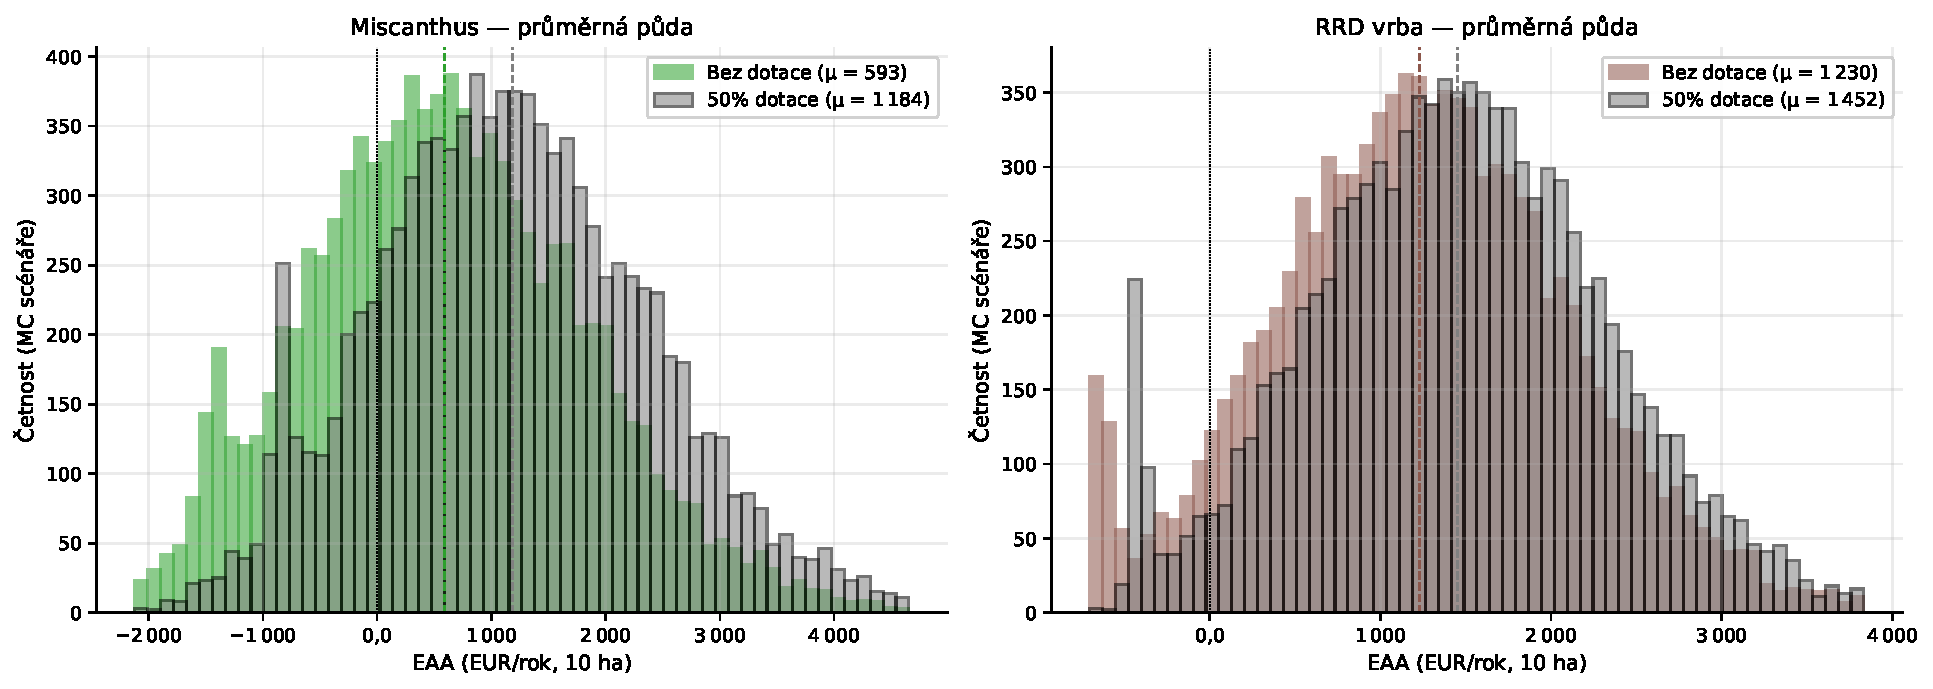
\includegraphics[width=\textwidth]{img/kap05/05_dotace_prumerna_eaa.pdf}
\caption{Posun rozdělení EAA na~průměrné půdě při~dotaci 50~\% CAPEX
(barevně) versus baseline bez~dotace (šedě). Tvar histogramu se~zachovává;
distribuce je~rigidně posunuta doprava o~konstantní translační vektor.}
\label{fig:dotace-eaa-prumerna}
\end{figure}

\paragraph{Závěr sekce.}
Z~hlediska \emph{střední ekonomické výnosnosti} je~kapitálová dotace
nejúčinnější u~marginálních půd (Neúrodná, Průměrná), kde posouvá
distribuci přes~nulovou hranici. Z~hlediska \emph{rizikového profilu}
však jde~o~nástroj s~omezenou efektivitou: nesnižuje variabilitu,
nezužuje chvost ani neeliminuje pravděpodobnost havárie plantáže
(která zůstává $p_f = 5~\%$). Nemůže proto kompenzovat strukturálně
nevhodné podmínky (Nevhodná půda zůstává ztrátová i~při~75~\% dotaci).
Skutečná \emph{rizikově orientovaná} podpora by~musela cílit
buď~na~stranu výnosů (cenová garance) nebo na~ohraničení chvostu
(parametrické pojištění proti suchu, kompenzace katastrof).

% ============================================================
\section{Katastrofický scénář -- ztracená dekáda}
\label{sec:katastrofa}

Baseline simulace v~kapitole~\ref{chap:vysledky} modeluje stochastické
počasí s~bodovými klimatickými stresy o~pravděpodobnosti $p_w = 5~\%$
a~půlením výnosu v~zasaženém roce. Tento mechanismus dobře zachycuje
\emph{občasné} extrémní události, ale~podceňuje scénář
\emph{klimaticky nepříznivého období}: sériu let s~dlouhotrvajícím
suchem, vysokými letními teplotami nebo opakovaným patogeny. Předpokládejme
projekci IPCC AR6 (scénáře SSP3-7.0 nebo~SSP5-8.5), kdy se~v~ČR
zvýší frekvence několikaletých period sucha a~tepelných vln.
Empirické studie klimatických dopadů na~zemědělství střední Evropy
ukazují, že~výnos plodin v~takovém období dlouhodobě klesá na~$40$--$60~\%$
regionálního průměru, aniž by~následoval rychlý návrat k~normálu.

\paragraph{Specifikace scénáře.}
Modelujeme jednorázovou sérii deseti po~sobě jdoucích let, kdy je~výnos
v~daném roce násoben nezávislým náhodným faktorem
\(\xi_t \sim \mathrm{Uniform}(0{,}40, 0{,}60)\), $t = t_0, \dots, t_0 + 9$.
Tato \emph{katastrofická dekáda} je~uniformně umístěna v~produkční fázi
plantáže (po~$n_{\mathrm{setup}} = 3$ letech, před~likvidační fází
u~SRC). Náhodné umístění zachycuje, že~pěstitel \emph{nemůže katastrofu
předvídat ani načasovat}; nezávislost faktorů $\xi_t$ navíc reflektuje
neúplnou predikovatelnost \emph{vnitřku} dekády (každý rok dílčí variabilita
i~uvnitř krize).

Scénář se~aplikuje navíc k~baseline stochastickým mechanismům
(klimatický stres $p_w$, OU proces ceny, riziko selhání plantáže $p_f$),
nikoli místo~nich -- jde o~\emph{kondicionálně horší světa}.

\subsection{Výsledky}
\label{subsec:katastrofa-vysledky}

\begin{table}[H]
\centering
\caption{Vliv katastrofické dekády (10~let, faktor 0,4--0,6) na~rizikový
profil. Změny vůči~baseline z~kapitoly~\ref{chap:vysledky}.}
\label{tab:katastrofa-shrnuti}
\renewcommand{\arraystretch}{1.15}
\small
\begin{tabular}{ll|rrrr|rrr}
\toprule
& & \multicolumn{4}{c|}{\textbf{Baseline}} & \multicolumn{3}{c}{\textbf{Katastrofa, změna $\Delta$}} \\
\textbf{Půda} & \textbf{Plodina} & $\mu_{\mathrm{EAA}}$ & $P(\!+\!)$ & CVaR$_{5\%}$ & $\sigma_\mathrm{CF}$ & $\Delta\mu$ & $\Delta P(\!+\!)$ & $\Delta$CVaR \\
\midrule
Nevhodná   & Miscanthus & $-3\,715$ & $0~\%$    & $-4\,843$ & $5\,892$ & $-248$    & $0$           & $-36$ \\
           & SRC vrba   & $-2\,565$ & $0~\%$    & $-3\,352$ & $3\,045$ & $-202$    & $0$           & $-15$ \\
\midrule
Neúrodná   & Miscanthus & $-1\,945$ & $0{,}1~\%$  & $-3\,080$ & $6\,454$ & $-667$    & $-0{,}1$~p.b.   & $-491$ \\
           & SRC vrba   & $-1\,049$ & $1{,}4~\%$  & $-1\,905$ & $5\,314$ & $-588$    & $-1{,}4$~p.b.   & $-405$ \\
\midrule
Průměrná   & Miscanthus & $+589$    & $67{,}2~\%$ & $-1\,676$ & $7\,498$ & $-1\,266$ & $\boldsymbol{-44{,}3}$~p.b. & $-763$ \\
           & SRC vrba   & $+1\,250$ & $92{,}1~\%$ & $-576$    & $8\,948$ & $-1\,103$ & $-35{,}9$~p.b.  & $-494$ \\
\midrule
Optimální  & Miscanthus & $+2\,871$ & $97{,}1~\%$ & $-515$    & $8\,573$ & $-1\,807$ & $-10{,}7$~p.b.  & $-620$ \\
           & SRC vrba   & $+3\,159$ & $97{,}5~\%$ & $+298$    & $12\,385$ & $-1\,547$ & $-0{,}6$~p.b.   & $-554$ \\
\bottomrule
\end{tabular}
\end{table}

\begin{figure}[H]
\centering
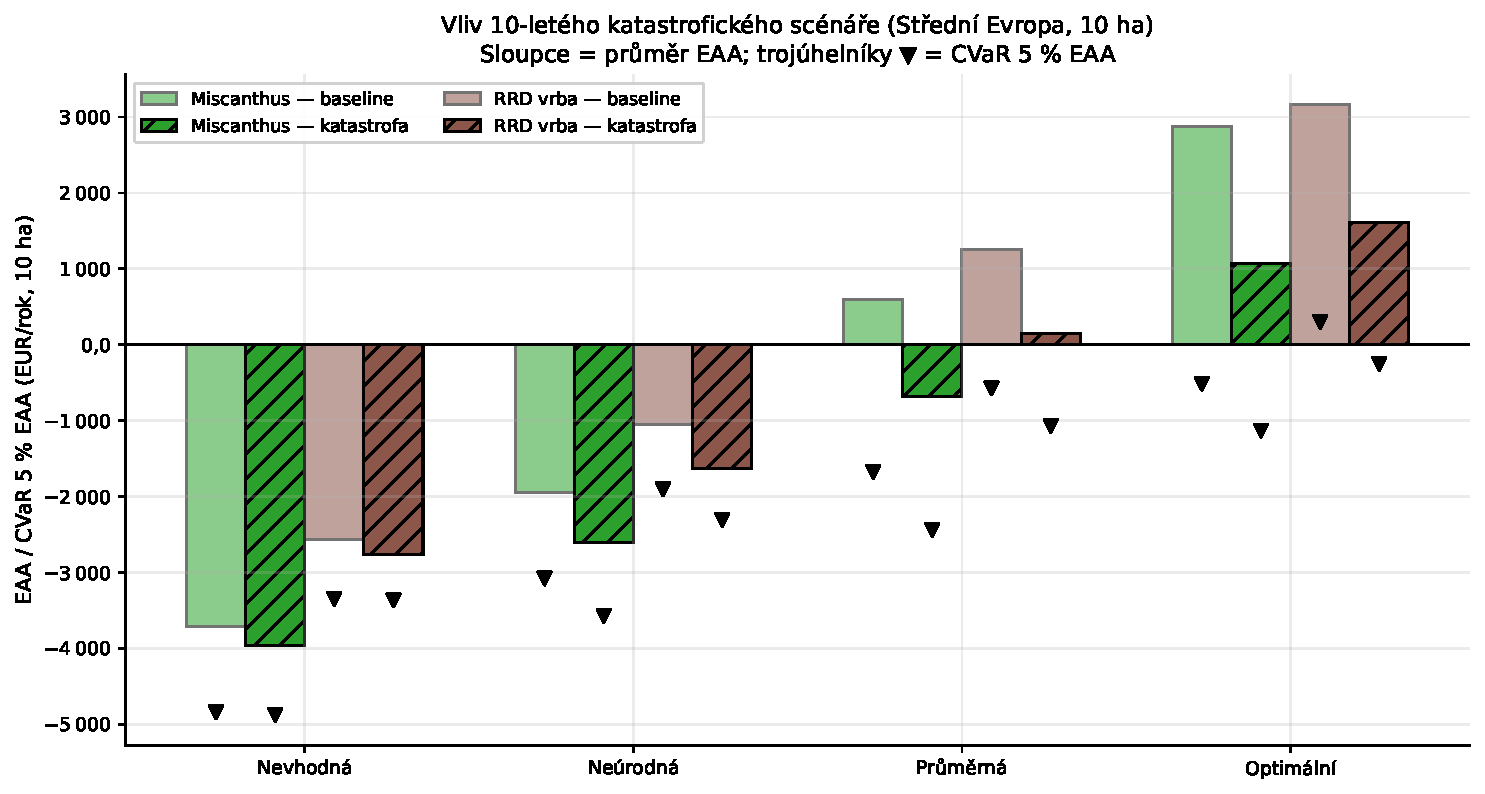
\includegraphics[width=\textwidth]{img/kap05/05_katastrofa_bars.pdf}
\caption{Posun průměrné EAA (sloupce) a~CVaR$_{5\%}$ (trojúhelníky) při
aplikaci katastrofické dekády. Trojúhelníky indikují, že~chvost rozdělení
se~prohlubuje a~vůči~průměru zůstává relativně stejně daleko.}
\label{fig:katastrofa-bars}
\end{figure}

\paragraph{Asymetrický dopad podle kvality půdy.}
Reakce rizikového profilu na~katastrofu je~výrazně \emph{nelineární}:
nevhodná půda absorbuje katastrofu téměř bez~efektu na~strukturální
rizikový profil, neboť baseline výnosnost je~tak nízká, že~"ztratit
něco, co~beztak prakticky není" má~malý absolutní dopad
($-248$~EUR/rok pro~Miscanthus). Naopak \emph{průměrná půda zachycuje
nejdramatičtější změnu pravděpodobnosti ziskovosti}: pro~Miscanthus
$P(\mathrm{EAA}>0)$ klesá ze~$67{,}2~\%$ na~$22{,}9~\%$, tj.~o~$44$
procentních bodů, a~projekt z~marginálně rentabilního přechází
do~ztrátového. SRC vrba na~průměrné půdě ztrácí $36$ procentních bodů
$P(+)$, ale~zůstává s~$56{,}2~\%$ pravděpodobností v~ziskovém pásmu.

Optimální půda zachovává robustní ziskovost ($P(+) = 86{,}4~\%$~/ $96{,}9~\%$),
přestože střední EAA klesá o~$1\,500$--$1\,800$ EUR/rok. Zde se~projevuje
\emph{strukturální rezerva}: vysoké výnosy nad~hraničním bodem
ziskovosti udržují distribuci v~pozitivním pásmu i~při~hluboké
klimatické krizi.

\paragraph{Asymetrie Miscanthus versus SRC vrba.}
Pro~všechny kvality půdy je~katastrofa pro~Miscanthus relativně
\emph{tvrdší} než pro~SRC. Důvod je~mechanický: Miscanthus se~sklízí
\emph{každoročně}, takže ztracený rok = ztracená sklizeň. SRC vrba se~sklízí
v~tříletých rotacích, a~i~kdyby v~jednom roce z~tříletého cyklu klesl
přírůstek, nadrůst v~ostatních letech může částečně kompenzovat. Proto
SRC vrba na~průměrné půdě ztrácí o~$8$ procentních bodů $P(+)$ méně
než Miscanthus.

Tato \emph{strukturální robustnost} SRC vrby vůči~klimatickým krizím
je~důležitý argument pro~diverzifikaci: i~kdyby Miscanthus měl~v~baseline
vyšší střední rentabilitu, SRC vrba zachovává ziskovost v~horších scénářích.
Tento bod přivádí k~analýze portfoliové diverzifikace
v~\S~\ref{sec:diverzifikace}.

\paragraph{Detailní distribuce.}
Obrázek~\ref{fig:katastrofa-grid} ukazuje histogramy EAA pro~všechny
kombinace půda~$\times$~plodina; ilustruje, jak~se~celé rozdělení posouvá
doleva, ale~zachovává si~svůj základní tvar (rozptyl $\sigma_\mathrm{CF}$
se~pouze mírně snižuje, protože ve~zranitelné dekádě jsou výnosy
v~"sníženém pásmu" relativně homogenní).

\begin{figure}[H]
\centering
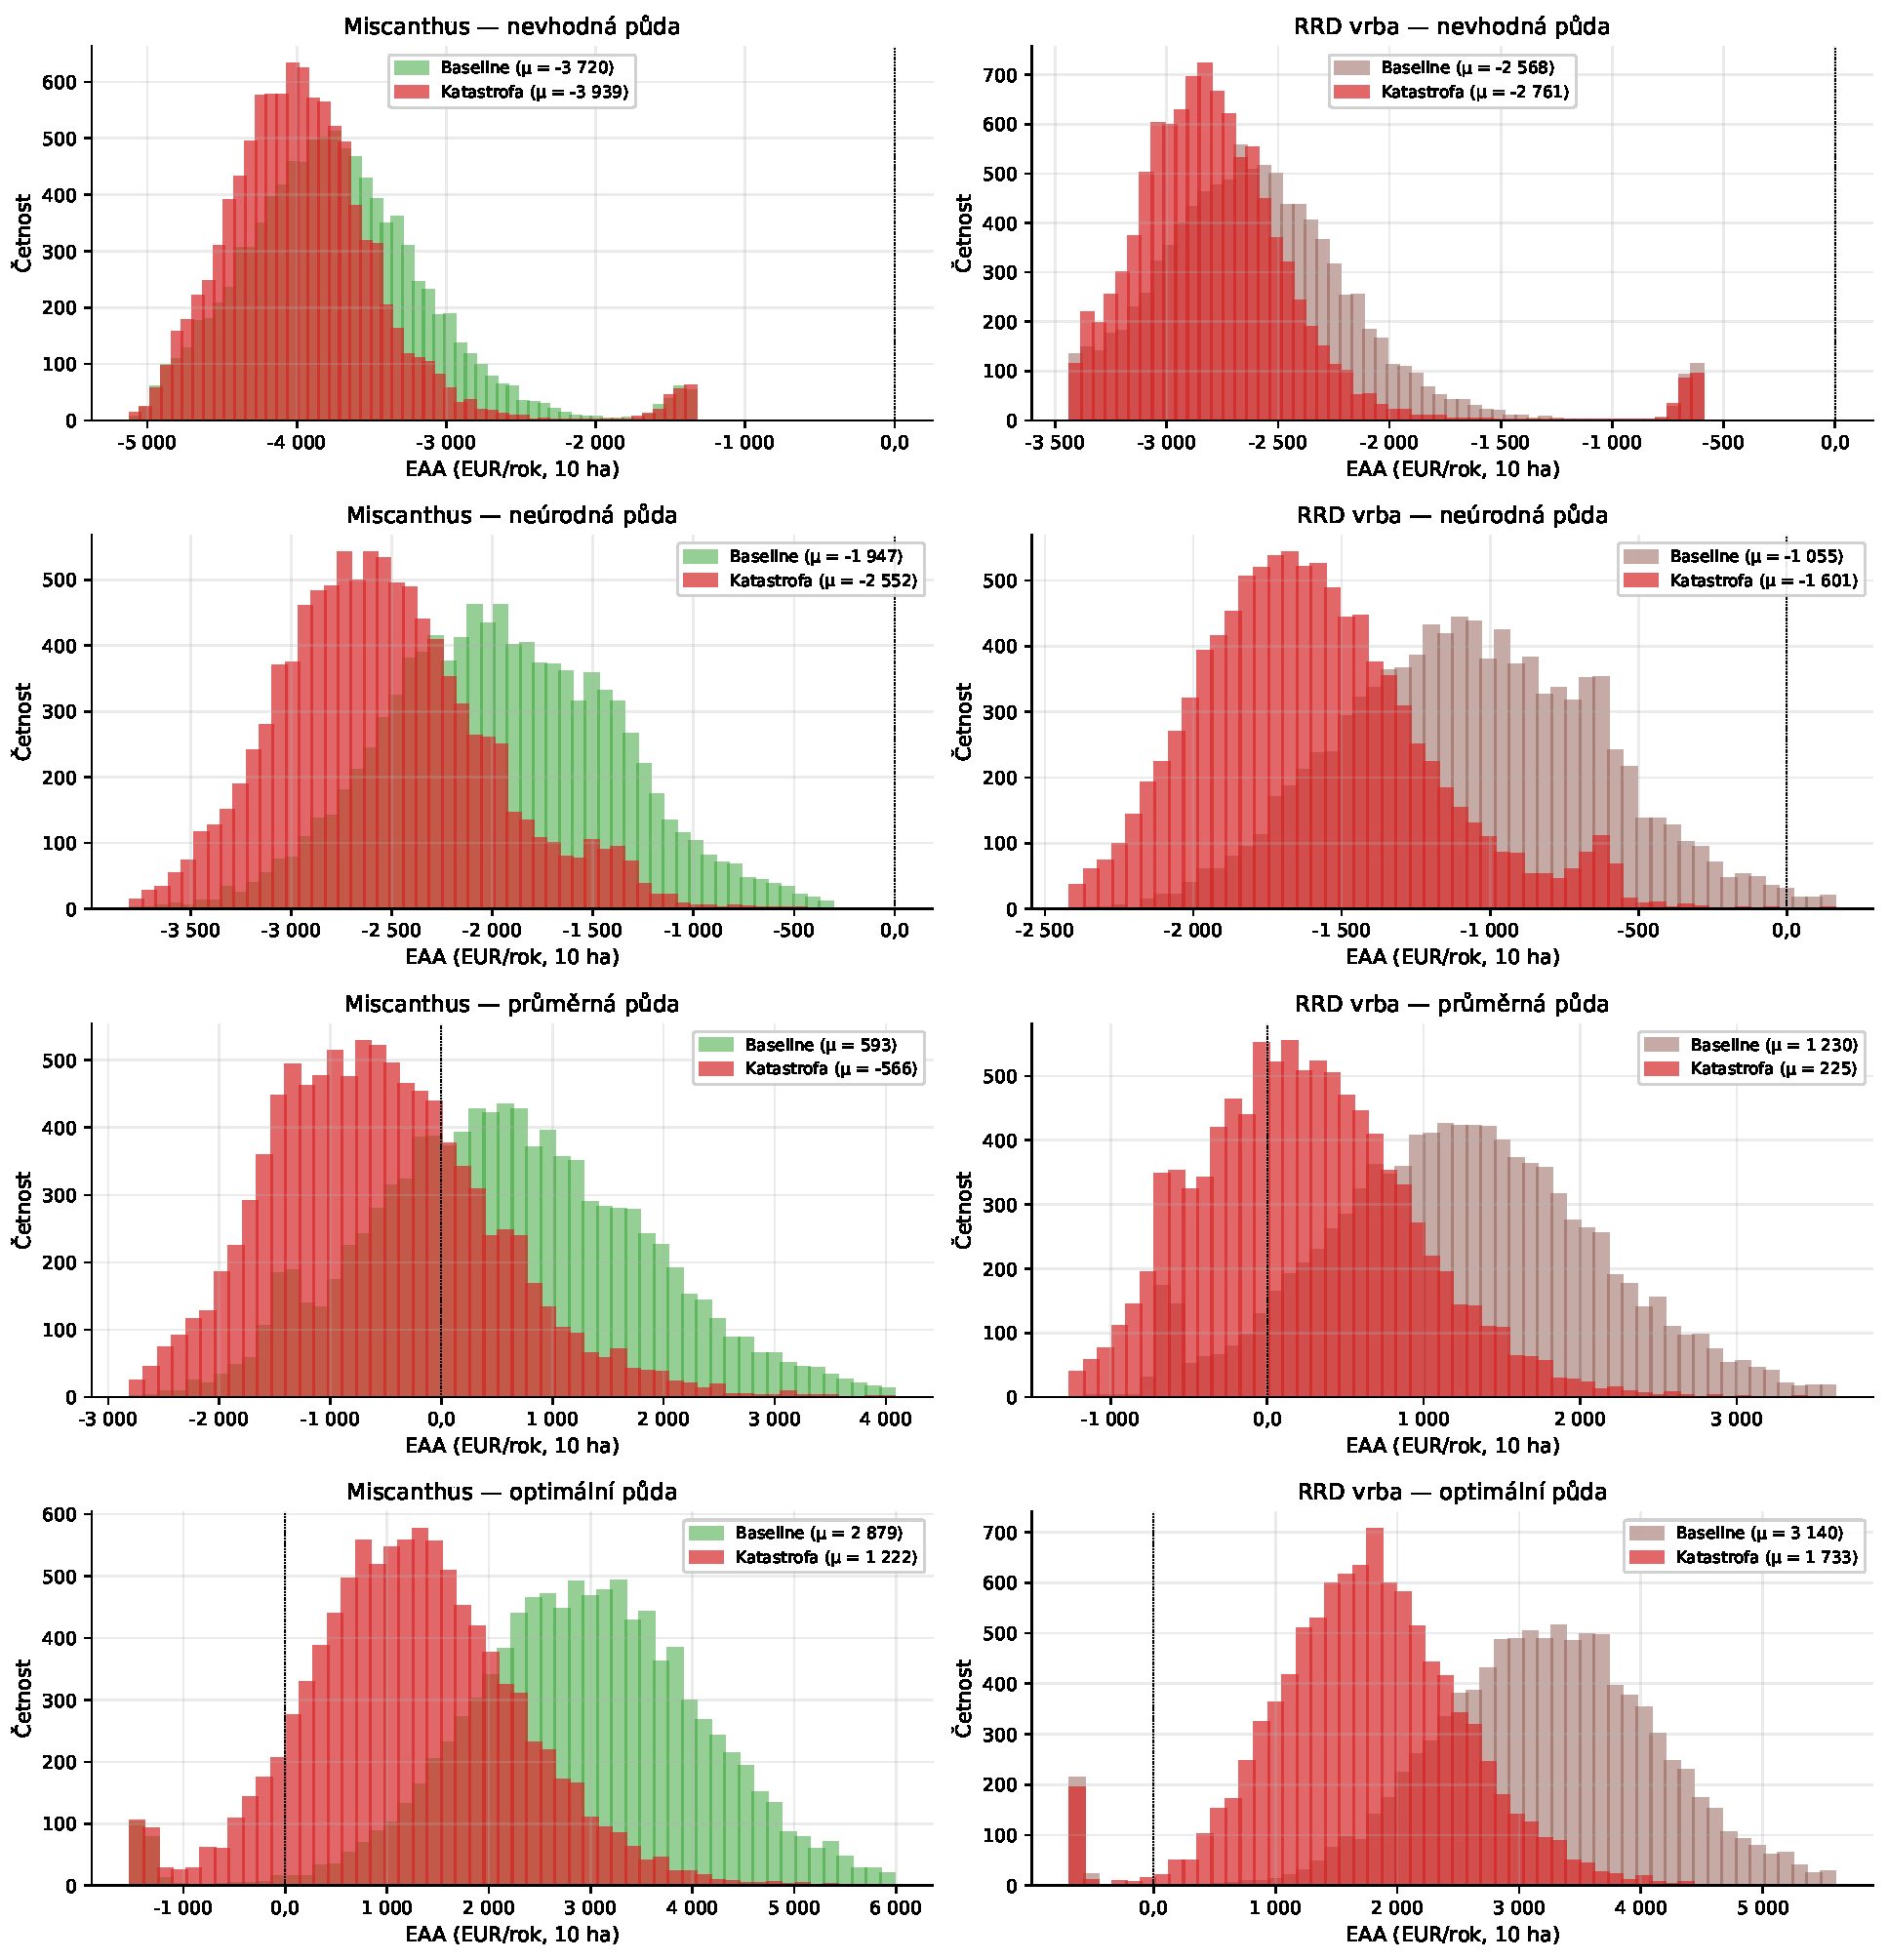
\includegraphics[width=\textwidth,height=0.78\textheight,keepaspectratio]{img/kap05/05_katastrofa_eaa_grid.pdf}
\caption{Rozdělení EAA pro~všechny kombinace půda~$\times$~plodina:
baseline (zeleně/hnědě) a~katastrofický scénář (červeně). Kritické
přechody přes~nulu jsou viditelné u~průměrné půdy.}
\label{fig:katastrofa-grid}
\end{figure}

\paragraph{Závěr sekce.}
Klimaticky podmíněná \emph{ztracená dekáda} je~scénář, který baseline
model výrazně podceňuje. Z~hlediska adaptace pěstitele má~několik
implikací:
\begin{itemize}
\item \textbf{Půdní strategie:} optimální půdy jsou~odolnější, ale~nevyhnou
      se~poklesu rentability. Strategie "zaplň nejhorší půdu prvně" je~tudíž
      kontraproduktivní -- biomasa na~nevhodné půdě je~strukturálně ztrátová
      i~před~katastrofou a~katastrofa její profil prakticky nezhorší.
\item \textbf{Druhová strategie:} SRC vrba je~v~katastrofě robustnější
      díky tříletému sklizňovému cyklu. Diverzifikace plantáže napříč
      oběma druhy snižuje očekávanou ztrátu (kvantifikováno v~\S~\ref{sec:diverzifikace}).
\item \textbf{Kompenzační nástroje:} dotace 50~\% CAPEX (\S~\ref{sec:dotace})
      přidává $\sim +300$ EUR/rok, zatímco katastrofa odebírá
      $\sim -1\,500$~EUR/rok na~optimální půdě. \emph{Dotace tedy nestačí
      katastrofu kompenzovat.} Adekvátním nástrojem by~bylo
      parametrické pojištění proti suchu (např.~vázané na~SPEI nebo
      teplotní index), které~by~přímo snižovalo CVaR.
\end{itemize}

% ============================================================
\section{Diverzifikace portfolia}
\label{sec:diverzifikace}

V~baseline analýze v~kapitole~\ref{chap:vysledky} jsme porovnávali
Miscanthus a~SRC vrbu \emph{samostatně} -- jako alternativní volby
pěstitele. V~praxi však vlastník 10~ha pole nemusí být nucen volit
\emph{buď}: může se~rozhodnout pěstovat \emph{obě} plodiny v~určitém
poměru, čímž vytváří \emph{portfolio} energetických plodin. Pokud
jejich~stochastika není perfektně korelovaná, klasická Markowitzova
teorie portfolia \citep{Markowitz1952} říká, že~kombinace dvou aktiv
\emph{snižuje} variabilitu výnosu i~chvostové riziko vůči~rizikově-vážené
průměrné individuální variabilitě.

V~této sekci kvantifikujeme efekt diverzifikace na~Průměrné a~Optimální
půdě. Definujeme váhu Miscanthusu $w_M \in [0, 1]$ a~váhu SRC vrby
$w_S = 1 - w_M$. Portfolio EAA je~dáno jako konvexní kombinace
\[
\mathrm{EAA}_p = w_M \cdot \mathrm{EAA}_M + w_S \cdot \mathrm{EAA}_S.
\]
Pro~konzistentní stochastiku používáme \emph{tytéž realizace klimatu
i~ceny} pro~oba druhy v~rámci jednoho scénáře (společný shock-driver),
což zohledňuje, že~plantáže obou plodin sdílí jednu lokalitu a~jeden
trh.

\subsection{Korelace a~efektivní hranice}
\label{subsec:portfolio-hranice}

Empirické korelace EAA mezi~Miscanthusem a~SRC vrbou v~rámci jedné
půdy:
\[
\rho_{M,S}^{\text{Průměrná}} = 0{,}68, \qquad
\rho_{M,S}^{\text{Optimální}} = 0{,}37.
\]
Vyšší korelace na~Průměrné půdě reflektuje fakt, že~v~hraničních
podmínkách je~rentabilita obou plodin společně determinována stejnými
makro faktory (cena, klimatický stres). Na~Optimální půdě, kde má~SRC
strukturálně lepší cash-flow profil (díky tříletým peakovým sklizňům
a~nižšímu CAPEXu), tlačí specifický mechanismus jejího cash flow
proti pravidelnému ročnímu toku Miscanthusu, což~vede k~podstatně nižší
korelaci. \emph{Tato nízká korelace je~ekonomický základ smysluplnosti
diverzifikace.}

\begin{figure}[H]
\centering
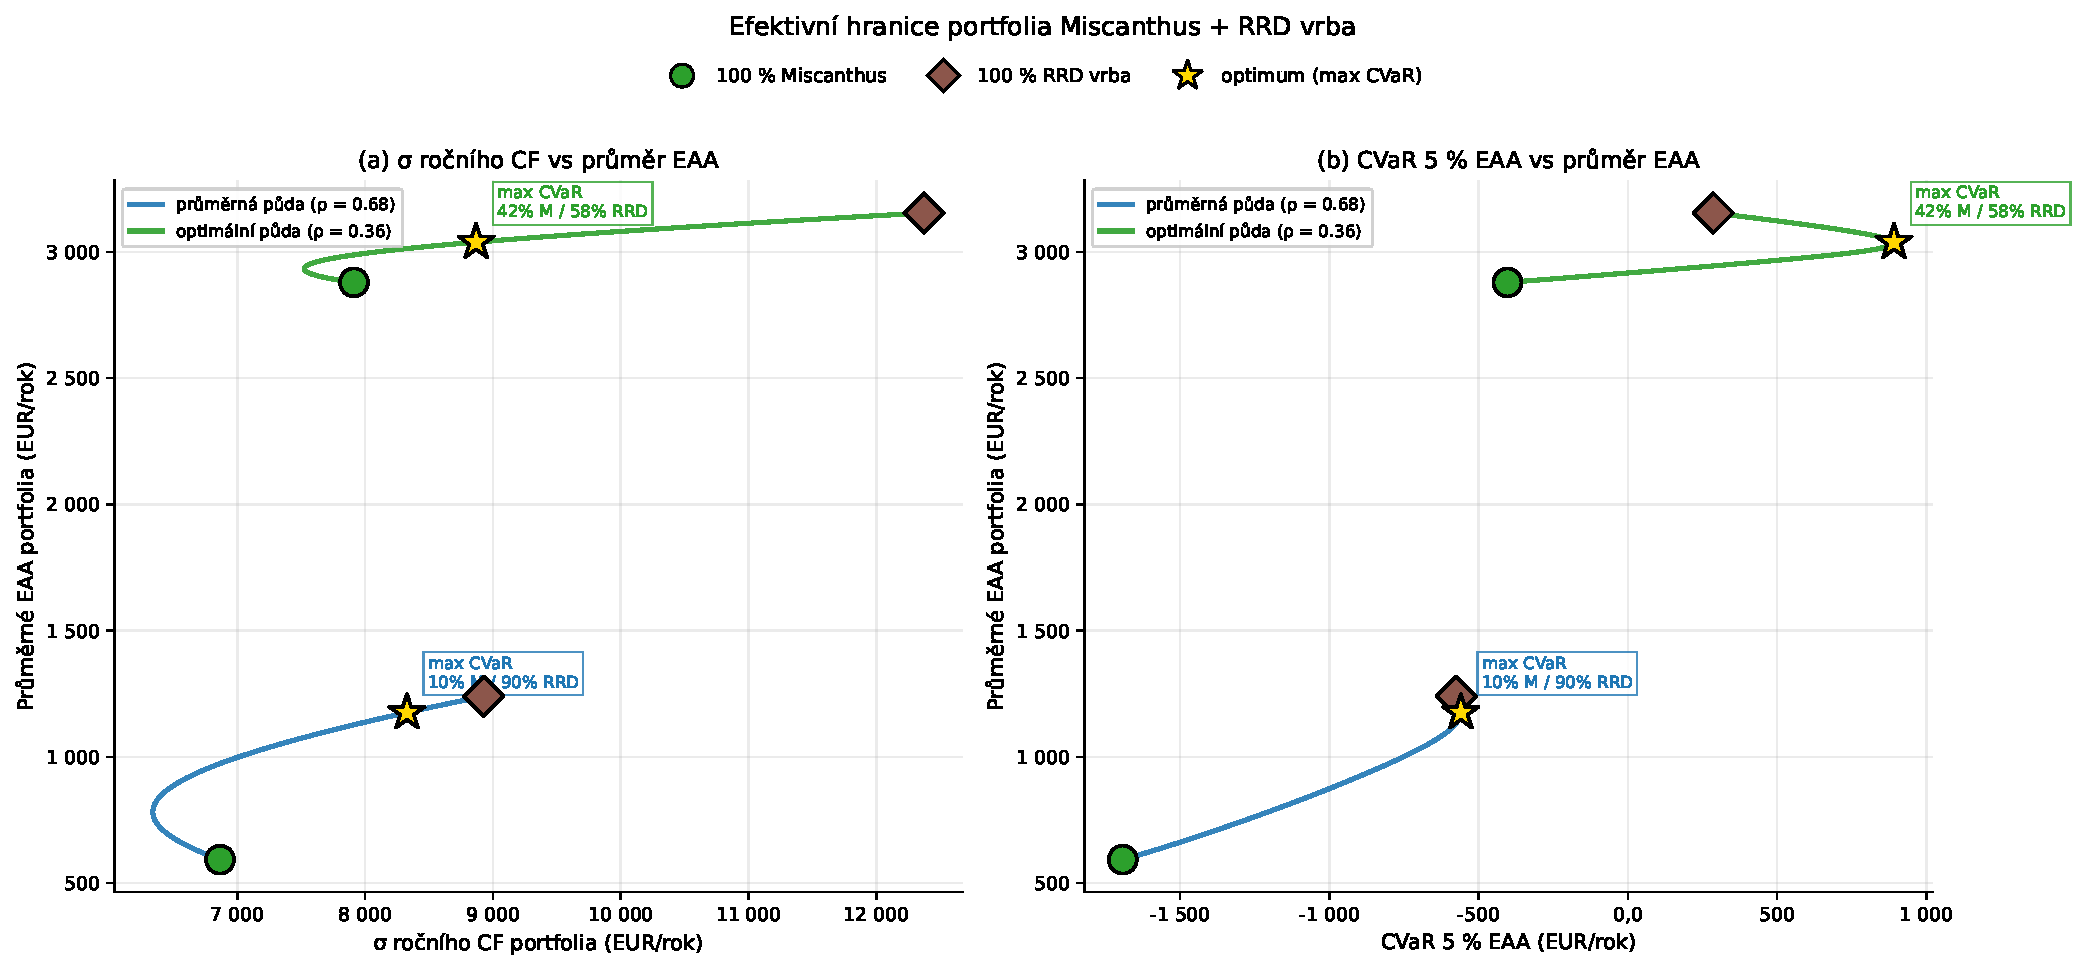
\includegraphics[width=\textwidth]{img/kap05/05_diverzifikace_hranice.pdf}
\caption{Efektivní hranice portfolia $w_M \cdot M + (1{-}w_M) \cdot S$
v~prostoru (a)~Markowitz $\mu$--$\sigma$ a~(b)~downside $\mu$--CVaR$_{5\%}$.
Hvězda značí optimální portfolio (minimum-variance vlevo, maximum-CVaR
vpravo); kosočtverec~$=$ 100~\% SRC; kolečko~$=$ 100~\% Miscanthus.}
\label{fig:diverzifikace}
\end{figure}

\subsection{Optimální složení portfolia}
\label{subsec:opt-portfolio}

\begin{table}[H]
\centering
\caption{Klíčové portfoliové statistiky pro~Průměrnou a~Optimální půdu.
\(w_M = 0\) značí 100~\% SRC, \(w_M = 1\) značí 100~\% Miscanthus.}
\label{tab:diverzifikace}
\renewcommand{\arraystretch}{1.15}
\small
\begin{tabular}{ll|rrrr}
\toprule
\textbf{Půda} & \textbf{Portfolio} & $\mu_{\mathrm{EAA}}$ & $\sigma_{\mathrm{EAA}}$ & CVaR$_{5\%}$ & $P(\!+\!)$ \\
\midrule
\multirow{4}{*}{Průměrná}
 & 100~\% Miscanthus ($w_M = 1$)         & $+589$    & $1\,234$ & $-1\,676$ & $67{,}2~\%$ \\
 & 100~\% SRC vrba ($w_M = 0$)           & $+1\,232$ & $890$    & $-582$    & $92{,}1~\%$ \\
 & Min $\sigma$ ($w_M = 5~\%$)           & $+1\,200$ & $888$    & $-573$    & $91{,}4~\%$ \\
 & Max CVaR ($w_M = 10~\%$)              & $+1\,168$ & $890$    & $-569$    & $90{,}6~\%$ \\
\midrule
\multirow{4}{*}{Optimální}
 & 100~\% Miscanthus ($w_M = 1$)         & $+2\,871$ & $1\,310$ & $-515$    & $97{,}1~\%$ \\
 & 100~\% SRC vrba ($w_M = 0$)           & $+3\,143$ & $1\,074$ & $+302$    & $97{,}5~\%$ \\
 & Min $\sigma$ ($w_M = 35~\%$)          & $+3\,048$ & $\mathbf{967}$ & $+831$ & $\mathbf{99{,}8~\%}$ \\
 & Max CVaR ($w_M = 40~\%$)              & $+3\,034$ & $970$    & $\mathbf{+861}$    & $\mathbf{99{,}9~\%}$ \\
\bottomrule
\end{tabular}
\end{table}

\paragraph{Optimální půda -- diverzifikační efekt je~zásadní.}
Smíšené portfolio $\sim 40~\%$~M~$+ 60~\%$~S na~optimální půdě:
\begin{itemize}
\item snižuje volatilitu o~$10~\%$ proti~čisté SRC vrbě
      ($\sigma$: $1\,074 \to 967$ EUR/rok),
\item téměř ztrojnásobuje pozitivní část chvostu (CVaR: $+302 \to +861$
      EUR/rok),
\item zvyšuje pravděpodobnost ziskovosti z~$97{,}5~\%$ na~$99{,}9~\%$ ---
      pouze 1 z~1\,000 scénářů končí ztrátou.
\end{itemize}
Náklad za~tuto stabilizaci je~mírný pokles průměrné EAA z~$3\,143$ na~$3\,034$
EUR/rok ($-3~\%$). Tento poměr "stabilita/ziskovost" je~mimořádně
příznivý a~plně potvrzuje hypotézu, že~v~biomasovém pěstování
\emph{platí klasické pravidlo diverzifikace}.

\paragraph{Průměrná půda -- diverzifikace marginální.}
Na~průměrné půdě je~optimální portfolio $w_M \approx 5$--$10~\%$ ---
prakticky čistá SRC vrba s~minimální Miscanthus přimíchanou pro~jemné
ladění variability. Důvod je~dvojí:
\begin{enumerate}
\item Vysoká korelace ($0{,}68$) snižuje benefitý křížového hedgingu --
      v~obou plodinách dochází k~podobným šokům současně.
\item SRC vrba má~na~průměrné půdě \emph{strukturální dominantnost} ve~všech
      ukazatelích (vyšší $\mu$, nižší $\sigma$, méně negativní CVaR,
      vyšší $P(+)$). Markowitzova diverzifikace pomáhá pouze tehdy, když~je~mezi
      aktivy \emph{trade-off}; zde je~však SRC vrba \emph{efficient}
      ve~všech dimenzích.
\end{enumerate}

\subsection{Praktická doporučení}
\label{subsec:portfolio-doporuceni}

Z~pohledu pěstitele s~10~ha pole:
\begin{itemize}
\item \textbf{Optimální půda:} ideální je~smíšené portfolio
      $\sim 4$~ha Miscanthus $+ 6$~ha SRC vrba (poměr 40~\%~/~60~\%).
      Tento poměr maximalizuje stabilitu při~jen mírném pokladu
      na~průměrné výnosnosti.
\item \textbf{Průměrná půda:} čistá SRC vrba je~ekonomicky efektivní
      volba; přimíchání Miscanthusu má~jen marginální vliv. Pokud
      pěstitel preferuje stabilní každoroční tržby (likviditní omezení),
      může zvolit část plochy s~Miscanthusem za~cenu mírně
      vyššího rizika.
\item \textbf{Klimatická adaptace:} v~kontextu katastrofického scénáře
      (\S~\ref{sec:katastrofa}) má~smíšené portfolio dodatečnou výhodu --
      SRC vrba s~tříletým rotačním cyklem absorbuje 10-letou ztracenou
      dekádu lépe než ročně sklízený Miscanthus, takže biologická
      diverzita rozšiřuje finanční diverzifikaci do~strukturální odolnosti.
\end{itemize}

\paragraph{Limitace.}
Naše analýza předpokládá, že~obě plodiny pěstované v~jedné lokalitě sdílí
\emph{tytéž} klimatické a~tržní šoky -- proto byla v~simulaci
synchronizována stochastika. V~realitě by~mohlo dojít k~ještě silnější
ko-pohyby (sucho ovlivní obě plodiny společně), nebo k~rozdílům
plynoucím z~prostorové variability ($M$ a~$S$ na~různých polích uvnitř
hospodářství). Analýza také nezahrnuje \emph{operační} aspekty
diverzifikace -- vyšší koordinaci sklizní, dvojí strojový park,
diverzifikované odběratele biomasy, které~by~mohly přinést další
benefity nebo náklady.

% ============================================================
\section{Limitace modelu a~doporučení pro~budoucí výzkum}
\label{sec:limitace}

Předložený stochastický Monte Carlo model představuje robustní
kvantitativní rámec pro~hodnocení rizikového profilu pěstování
energetických plodin v~ČR. Přesto má~pochopitelně řadu \emph{limitací}
plynoucích z~přijatých zjednodušujících předpokladů. V~následujícím
přehledu shrnujeme nejvýznamnější z~nich a~navrhujeme směry,
v~nichž by~budoucí výzkum mohl model dále rozšířit.

\subsection{Limitace stochastiky}
\label{subsec:lim-stoch}

\paragraph{Stacionarita klimatu.}
Mechanismus klimatického stresu je~modelován jako \emph{stacionární}
procesy: weather multiplier ($w_t \sim \mathcal{LN}(0, \sigma_w)$
omezený na~$[0{,}5; 1{,}5]$) a~Bernoulliův klimatický stres
($p_w = 5~\%$) jsou~nezávislé na~čase. V~realitě se~však klima
projektuje jako \emph{nestacionární}: SSP scénáře IPCC AR6 (2021) předpokládají
zhoršování suchových režimů a~prodlužování heat-wave epizod
i~v~podmínkách střední Evropy. Jednoduchá implementace nestacionarity by~spočívala
v~lineárním nárůstu $\sigma_w(t) = \sigma_w^0 + g_\sigma \cdot t$
nebo $p_w(t) = p_w^0 \cdot (1 + g_p \cdot t)$. Sekce~\ref{sec:katastrofa}
implementuje speciální variantu této úvahy (sériová ztracená dekáda),
ale~pokrytí celého spektra adaptace by~vyžadovalo systematickou
nestacionární kalibraci.

\paragraph{Korelační struktura.}
Baseline model nastavuje korelaci mezi~počasím a~cenou
biomasy na~$\rho = 0$ (neutrální baseline). Empirická data však naznačují,
že~by~tato korelace mohla být \emph{záporná}: suché roky obvykle vedou
k~nižší úrodě biomasy (přírody i~konkurujících zemědělských plodin),
což zvyšuje vzájemnou cenu. Implementační framework je~připraven
(Choleskyho dekompozice + Gaussovská kopule, viz~kapitola~\ref{chap:metodologie}),
ale~kalibrace $\rho$ z~ČR-specifických dat (např.~ČHMÚ + ERÚ)
by~byla samostatným úkolem.

\paragraph{Tail-skewness.}
Použití normální (resp.~lognormální) distribuce pro~weather multiplier
i~OU proces ceny předpokládá \emph{symetrické} chvosty. Realita však
ukazuje, že~klimatické extrémy mají~výrazně \emph{těžší levý chvost}
(tail-fattening). Adekvátnější modely zahrnují~Studentovu $t$-distribuci
(s~nízkými stupni volnosti), generalizovanou Pareto distribuci
nebo~přepínací Markovský~regime ($M_t$ pro~"normální" a~"krizové"
roky). Tyto modely by~zvýšily CVaR i~$P(\mathrm{NPV} < 0)$.

\subsection{Limitace ekonomického rámce}
\label{subsec:lim-ekon}

\paragraph{Statická cena na~začátku životnosti.}
Model přijímá počáteční prodejní cenu biomasy ($p_0$) jako exogenně
zadaný kalibrační parametr ($116$ EUR/t~DM Miscanthus, $128$ EUR/t~DM SRC).
Reálná tvorba ceny biomasy v~ČR je~však \emph{endogenní} -- závisí
na~regionálním poměru nabídka/poptávka, vzdálenosti k~odběrateli
(teplárna, výroba pelet), formě biomasy (rostlá / štěpka / pelety) atd.
Budoucí rozšíření by~mohlo zahrnout regionálně specifické cenové
indexy nebo dvouvrstvý model (tržní cena + transportní náklady).

\paragraph{Statický model nákladů.}
Eskalace OPEX je~modelována konstantní $2~\%$/rok, což odpovídá
historické inflační stopě 2010--2022. V~období~vyšší inflace
(2022--2024 ČR průměr $\sim 9~\%$) je~tento předpoklad nedostatečný.
Mohl by~být nahrazen~stochastickým~AR(1) procesem s~kalibrovanou
volatilitou nebo~Markovským regime-switching modelem (mírná inflace
vs.~vysoká inflace).

\paragraph{Pevná životnost.}
Modely předpokládají pevnou životnost plantáže ($25$ let Miscanthus,
$30$ let SRC). V~realitě \emph{rozhodnutí o~likvidaci} je~optimalizační
volba pěstitele -- pokud projekt není dlouhodobě rentabilní, mohlo
by~být ekonomicky efektivní likvidovat dřív. Model "abandonment option"
nebo přístup "real option valuation" (Dixit \& Pindyck, 1994) by~přidal
tomuto rozhodnutí dynamické rozměr.

\subsection{Limitace dotační analýzy}
\label{subsec:lim-dotace}

V~sekci~\ref{sec:dotace} jsme modelovali pouze \emph{kapitálovou} dotaci
formou jednorázového příspěvku k~CAPEXu. Reálná škála veřejné podpory
v~ČR je~však bohatší:
\begin{itemize}
\item \textbf{SZP přímé platby a~ekoschémata} (cca 230~EUR/ha/rok
      podle Strategického plánu SZP 2023--2027) -- modelovatelné
      jako stochasticky bez~variabilita, ale~pevný roční bonus.
\item \textbf{Garantovaná výkupní cena} (Vyhláška 315/2025~Sb.,
      Cenový výměr ERÚ 8/2025) -- redukuje volatilitu prodejní ceny
      na~spodní hranici, čímž~mění~tvar OU procesu.
\item \textbf{Modernizační fond} -- variabilní krytí v~závislosti
      na~konkrétním projektu.
\item \textbf{Pojištění proti suchu/katastrofě} -- parametrické
      indexované pojištění by~mělo modelovat výplatu jako
      $f(\mathrm{SPEI}_t)$ nebo $f(\Delta T_t)$.
\end{itemize}
Plná analýza interakce těchto nástrojů je~aktuální výzkumný úkol
(viz~např.~\citet{knapek_2024}).

\subsection{Limitace prostorového/agronomického modelu}
\label{subsec:lim-prostor}

\paragraph{Bodový model.}
Model zachází s~10ha plantáží jako s~\emph{bodovou} entitou bez~prostorové
heterogenity. V~realitě se~kvalita půdy mění i~v~rámci jednoho pole
(historie hnojení, mikroreliéf, drenážní podmínky), což by~vedlo
k~heterogennímu výnosu i~nákladům. Pro~větší plochy ($> 50$ ha)
je~třeba GIS-based přístup s~pixelovou resolucí.

\paragraph{Statický model dynamiky výnosu.}
Křivka přírůstku Miscanthusu (Křen 2018; ZD Vyšší Brod 2021)
i~Wegerova SRC křivka jsou~kalibrovány z~empirických dat, ale~předpokládají
\emph{deterministické} tvary závislé pouze na~čase. Realisticky
je~přírůstek funkcí kumulativního stresu, množství deště i~teploty
v~předchozích letech. Mohl by~být nahrazen biofyzikálním modelem
(např.~APSIM-Miscanthus, MISCANFOR), který~by~mapoval klimatické
vstupy přímo na~výnos.

\paragraph{Vstupní data o~výnosu pro~ČR.}
Modely pracují s~rozsahy $0$--$16$~t~DM/ha pro~Miscanthus a~$0$--$15$~t~DM/ha
pro~SRC podle kvality půdy, kalibrovanými z~Wegerových studií, dat
ZD Vyšší Brod a~doporučení VÚKOZ. Tyto rozsahy jsou~ČR-specifické,
ale~empirických dlouhodobých dat (>10 let) je~v~ČR poměrně málo.
Sběr dlouhodobých dat z~existujících plantáží by~zlepšil kalibraci.

\subsection{Doporučení pro~budoucí výzkum}
\label{subsec:budouci-vyzkum}

Na~základě výše uvedených limitací doporučujeme následující směry
budoucího výzkumu:
\begin{enumerate}
\item \textbf{Nestacionární klimatický modul:} integrace IPCC SSP scénářů
      do~stochastiky $\sigma_w(t), p_w(t)$, kalibrace na~česká pozorování
      ČHMÚ.
\item \textbf{Endogenní cenový model:} dvoudimenzionální cenový
      framework (tržní cena~$+$~transportní náklad), kalibrace z~ERÚ dat
      a~regionálních smluv s~teplárnami.
\item \textbf{Real-options framework:} explicitní modelování
      rozhodnutí pěstitele o~obnově / likvidaci v~průběhu života
      plantáže (typicky pomocí dynamického programování nebo Bellmanovy
      rovnice).
\item \textbf{Plná dotační analýza:} simulace všech v~ČR dostupných
      podpůrných nástrojů (SZP, Modernizační fond, Vyhláška 315/2025
      Sb., parametrické pojištění) a~jejich vzájemných interakcí.
\item \textbf{Bayesovská kalibrace:} aktualizace prior distribucí
      vstupních parametrů na~základě dlouhodobých pozorování (např.~3--5
      let dat z~existujících českých plantáží), což by~umožnilo
      \emph{posterior predictive check} a~validaci modelu.
\item \textbf{Globální citlivostní analýza:} doplnění OAT analýzy
      z~kapitoly~\ref{chap:vysledky} (\S~\ref{sec:vysledky-citlivost})
      o~Sobolovy indexy nebo metodu FAST, která~zachytí interakce parametrů.
\item \textbf{Agronomický biofyzikální modul:} náhrada deterministických
      růstových křivek empirickým biofyzikálním modelem (APSIM, MISCANFOR),
      který~by~přímo mapoval~klima na~výnos.
\end{enumerate}

\subsection{Klíčové závěry kapitoly}
\label{subsec:zaver-diskuse}

Diskuse v~této kapitole vedle prosté validace baseline výsledků přinesla
několik nových empirických zjištění, která~mají~přímý praktický význam
pro~rozhodování pěstitele i~tvůrce zemědělské politiky:
\begin{enumerate}
\item \textbf{Dotace 50~\% CAPEX} posouvá průměrnou EAA o~$+300$ EUR/rok
      (M)~/~$+225$ EUR/rok (S), ale~\emph{nezužuje rozdělení}. Pro~snížení
      \emph{rizikového} profilu jsou~účinnější nástroje cílené
      na~cenu nebo na~chvost (parametrické pojištění).
\item \textbf{Klimatická katastrofa (10 let snížených výnosů)}
      představuje největší riziko pro~Průměrnou půdu --
      Miscanthus zde ztrácí $44$ procentních bodů $P(+)$. Optimální
      půda zůstává robustní díky strukturální rezervě.
\item \textbf{Diverzifikace M~$+$~SRC dává smysl pouze na~Optimální půdě}
      (korelace $0{,}37$). Optimální poměr $\sim 40~\%$~M~$+ 60~\%$~S
      ztrojnásobuje CVaR z~$+302$ na~$+861$ EUR/rok a~zvyšuje $P(+)$
      na~$99{,}9~\%$. Na~Průměrné půdě dominuje SRC vrba ve~všech
      ukazatelích.
\end{enumerate}

Tyto závěry vedou k~přirozené generální syntéze v~závěrečné kapitole práce.
